\documentclass[10pt]{beamer}
\usetheme{Frankfurt}
\usecolortheme{dolphin}
\usepackage[utf8]{inputenc}
\usepackage[spanish]{babel}
\usepackage{amsmath}
\usepackage{amsfonts}
\usepackage{amssymb}
\usepackage{graphicx}
\usepackage{ragged2e}
\setbeamertemplate{navigation symbols}{} 
\author[Kevin García - Alejandro Vargas]{Kevin García 1533173 \newline Alejandro Vargas 1525953}
\institute{Universidad del Valle}
\title{Diseño y validación de muestreo de cítricos para detección de enfermedades en viveros del Valle del Cauca}

\newenvironment{changemargin}[2]{%
  \begin{list}{}{%
    \setlength{\topsep}{0pt}%
    \setlength{\leftmargin}{#1}%
    \setlength{\rightmargin}{#2}%
    \setlength{\listparindent}{\parindent}%
    \setlength{\itemindent}{\parindent}%
    \setlength{\parsep}{\parskip}%
  }%
  \item[]}{\end{list}}%

\newenvironment<>{varblock}[2][.9\textwidth]{%
  \setlength{\textwidth}{#1}
  \begin{actionenv}#3%
    \def\insertblocktitle{#2}%
    \par%
    \usebeamertemplate{block begin}}
  {\par%
    \usebeamertemplate{block end}%
  \end{actionenv}}


\newcommand\Wider[2][3em]{%
\makebox[\linewidth][c]{%
  \begin{minipage}{\dimexpr\textwidth+#1\relax}
  \raggedright#2
  \end{minipage}%
  }%
}
%\setbeamercovered{transparent} 
%\setbeamertemplate{navigation symbols}{} 
%\logo{} 
%\institute{} 
%\date{} 
%\subject{} 
\begin{document}
\begin{frame}[plain]
\maketitle
\end{frame}

\begin{frame}{Contenido}
\tableofcontents
\end{frame}

\section{Proyecto}
\begin{frame}
\frametitle{Información del proyecto}
\begin{block}{Entidad encargada}
\begin{itemize}
\justifying
\item AGROSAVIA (Corpoica)
~\\La Corporación Colombiana de Investigación Agropecuaria, Corpoica, es una entidad pública descentralizada de participación mixta sin ánimo de lucro, de carácter científico y técnico, cuyo objeto es desarrollar y ejecutar actividades de Investigación, Tecnología y transferir procesos de Innovación tecnológica al sector agropecuario.
\end{itemize}
\end{block}
\begin{block}{Personal a cargo}
\begin{itemize}
\item[-]Nubia Murcia Riaño (Investigador Ph.D.)
\item[-]Mauricio Fernando Martínez (Investigador Máster)
\item[-]Elizabeth Narvaez Toro (Líder de Seguimiento y Evaluación)
\end{itemize}
\end{block}
\end{frame}

\section{Problema}
\subsection{Problema contextual}
\subsection{Problema estadístico}
\begin{frame}
\begin{block}{Problema contextual}
\justifying
~\\Existen diversas enfermedades en los cítricos transmitidas principalmente por injertación, vectores (organismos o insectos), y uso de herramienta, las cuales son muy dañinas para este cultivo, entre ellas, el virus de la tristeza, HLB, Leprosis y Exocortis. Estas debilitan el árbol, generando producciones escasas, y en casos avanzados puede llegar a matar el árbol. El inconveniente es que estas enfermedades son asintomáticas en edades tempranas de la planta, es decir, no podemos diferenciar a simple vista una planta infectada con una no infectada. Al sembrar una planta con alguna de estas infecciones desde el comienzo, se perderá mucho dinero invirtiendo en su mantenimiento, por lo cuál se necesita asegurar o garantizar que las plantas que van a ser sembradas y entregadas estén limpias de estas enfermedades, logrando de esta manera la producción de material certificado.
\end{block}
\begin{block}{Problema estadístico}
\begin{itemize}
\justifying
\item ¿Es posible diseñar un plan de muestreo adecuado y asequible que permita la detección temprana de estas enfermedades en los cítricos?
\end{itemize}
\end{block}
\end{frame}


\section{Justificación}
\begin{frame}
\frametitle{Justificación}
\justifying
Desde el área de la estadística se han visto muchos estudios con lotes de cítricos criados en viveros los cuales se orientan a evaluar efectos que tienen ciertos tratamientos sobre las plantas,(para evaluar rendimiento, producción, crecimiento y muchos otros factores) pero muy pocos se orientan al muestreo, el cual cumple un papel muy importante ya que a partir de este se pueden tomar decisiones certeras. La implementación de un buen plan de muestreo en estos viveros definirá si un lote puede llegar a catalogarse como “bueno” o si por el contrario hay que descartarlo como un lote infectado.

\end{frame}

\section{Objetivos}
\subsection{Objetivos general}
\subsection{Objetivos específicos}
\begin{frame}
\frametitle{Objetivos propuestos}
\begin{block}{Objetivo general}
Diseñar y validar un plan de muestreo para aceptación y rechazo de lotes de cítricos en viveros del Valle del Cauca que permita estimar la cantidad de plantas infectadas en el lote.
\end{block}
\begin{block}{Objetivos específicos}
\begin{itemize}
\justifying
\item[-]Proponer y diseñar diferentes tipos de muestreo tipo aceptación/rechazo para lotes de cítricos en viveros del Valle del Cauca.
\item[-]Validar los diseños muéstrales por medio de simulación teniendo en cuenta confianza y costo del muestreo.
\item[-]Estimar la cantidad de plantas infectadas en el lote.
\end{itemize}
\end{block}
\end{frame}

\section{Variable de interés}
\begin{frame}
\frametitle{Variable de interés}
~\\Nuestra variable de interés se puede definir de la siguiente manera:
$$X= \left\{\begin{array}{cc}
             1 &   si \; la \; planta \; esta \; infectada \\
             \\ 0 &  si \; la \; planta \; no \; esta \; infectada \\
             \end{array}
   \right.$$
\end{frame}


\begin{frame}
\frametitle{Variable de interés}
~\\Para llegar a la variable de interés definida anteriormente, se lleva a cabo una prueba de laboratorio en la cuál se pueden medir hasta 45 muestras de tejido de plantas, donde se obtiene al final una coloración en el recipiente, a esta coloración se le hace una lectura visual o colorimétrica, usualmente se utiliza más la medida colorimétrica por ser mas objetiva, esta se obtiene con un valor de absorbancia, que corresponde en pocas palabras a una cuantificación de la percepción del color. Se encuentra de la siguiente manera:
\[ A_\lambda=-log_{10} \left( \frac{I}{I_0}\right) \]
~\\Donde:
~\\I es la intensidad de la luz con una longitud de onda específica $\lambda$ tras haber atravesado una muestra (intensidad de la luz transmitida).
~\\$I_0$  es la intensidad de la luz antes de entrar a la muestra (intensidad de la luz incidente).
\end{frame}

\section{Antecedentes}
\subsection{Antecedentes contextuales}
\begin{frame}
\frametitle{Antecedentes}
\Wider{
\begin{varblock}[12cm]{Antecedentes contextuales}
\begin{itemize}
\justifying
\item[1.]Epidemiología de Plum pox virus y citrus tristeza virus en bloques de plantas de vivero. Métodos de control.(2010)\cite{AC1}
~\\El objetivo de esta tesis fue el estudio de los distintos factores que determinan la epidemiología de PPV y CTV en vivero, con el fin de establecer posibles estrategias de control. Se utilizó un muestreo que consistía en dividir las parcelas en bloques estadísticos imaginarios(dos bloques de plantas) y finalmente se tomaron ciertas filas de plantas(4 primeras filas).
\item[2.]Enfermedades causadas por Phytophthora en viveros de plantas ornamentales.(2012)\cite{AC2}
~\\El objetivo de este trabajo fue estudiar las enfermedades causadas por las especies de Phytophthora. Se exploraron 23 viveros de plantas ornamentales, muestreando solamente plantas sintomáticas, analizando un total de 360 plantas.
\end{itemize}
\end{varblock}
}
\end{frame}

\begin{frame}
\frametitle{Antecedentes}
\Wider{
\begin{varblock}[12cm]{Antecedentes contextuales}
\begin{itemize}
\justifying
\item[3.]Phytophthora community structure analyses in Oregon nurseries inform systems approaches to disease management.(2014)\cite{AC3}
~\\El objetivo fue describir la estructura de las comunidades de Phytophthora en 4 viveros comerciales. Se tomaron muestras de los 4 viveros cada 2 meses durante 4 años, recolectando 5 plantas de cada género en cada fecha de muestreo. Se seleccionaron plantas sintomáticas.
\item[4.]El Virus de la Tristeza de los Citricos (CTV) en Plantaciones Comerciales y Viveros de la República Dominicana.(2008)\cite{AC4}
~\\Para este proyecto se tomaron muestras de 9 viveros y dentro de cada vivero se tomaron muestras del 1\% para lotes grandes y 2\% para lotes pequeños. Los lotes estaban en rangos de entre 2000 y 40000 plantas, se determino que el CTV incremento en más del 80\% desde los últimos 10 años.
\end{itemize}
\end{varblock}
}
\end{frame}

\begin{frame}
\frametitle{Antecedentes}
\Wider{
\begin{varblock}[12cm]{Antecedentes contextuales}
\begin{itemize}
\justifying
\item[5.]Ocurrencia de Huanglongbing (Candidatus Liberibacter asiaticus) y su vector Diaphorina citri Kuwayama (Hemiptera: Liviidae) en viveros de cítricos de Masaya.(2018)\cite{AC5}
~\\Para este experimento se tomaron plántulas de plantas en las cuales sus hojas presentaban síntomas de HLB, cada mes se tomaron 20 plántulas, al final se tenían 80 plántulas por vivero. Los resultados obtenidos fueron que para cada vivero la proporción de plantas infectadas con HLB era del 12.5\%, 25\%, 12.5\% y 25\% respectivamente.
\end{itemize}
\end{varblock}
}
\end{frame}

\subsection{Antecedentes estadísticos}
\begin{frame}
\frametitle{Antecedentes}
\Wider{
\begin{varblock}[12cm]{Antecedentes estadísticos}
\begin{itemize}
\justifying
\item[1.]Monitorización del cumplimiento del protocolo de mantenimiento de la cateterización venosa mediante el método LQAS.(2004)\cite{AE1}
~\\El objetivo fue evaluar el incumplimiento del mantenimiento de la cateterización venosa de un hospital mediante LQAS. Se evaluaron 4 criterios. Se partió de un estándar de cumplimiento del 95\% y un umbral mínimo del 85\%, un error a=5\% y un error b=20\%, se calculó un tamaño de muestra de 44 casos y el número minimo de cumplimientos del protocolo de 39.
\item[2.]Using lot quality assurance sampling to improve immunization coverage in Bangladesh.(2001)\cite{AE2}
~\\El objetivo fue determinar las áreas de baja cobertura vacunal en cinco ciudades de Bangladesh. En el primero, se seleccionó la meta del 85\% de cobertura como umbral superior y 60\% como umbral inferior, un nivel de confianza del 80\% y se encontró que el tamaño de muestra era de 13, y el número de aceptación sería de 9 niños. En el segundo, el umbral inferior fue de 60\% e inferior de 40\%, un nivel de confianza del 95\% y se encontró que el tamaño de muestra era de 16 niños.
\end{itemize}
\end{varblock}
}
\end{frame}


\begin{frame}
\frametitle{Antecedentes}
\Wider{
\begin{varblock}[12cm]{Antecedentes estadísticos}
\begin{itemize}
\justifying
\item[3.]Evaluación, mejora y monitorización de la adecuación de ingreso y estancia en Medicina Interna con el muestreo de aceptación de lotes.(2000)\cite{AE3}
~\\En este proyecto se utilizó el método de LQAS para evaluar la calidad, se tomaron muestras de pacientes en diferentes periodos primero evaluando la calidad del ingreso y estancia actual y luego tras hacer ciertas mejoras. Crearon un umbral de mala calidad que es “\% de adecuación” que funciona como regla de parada.
\item[4.]Field trial of applicability of lot quality assurance sampling survey method for rapid assessment of prevalence of active tracoma.(2003)\cite{AE4}
~\\Este proyecto utiliza el método de LQAS para clasificar niños que padecen de tracoma en 3 tres categorías de prevalencia, se crearon umbrales para determinar las categorías y basándose en datos de encuestas se decide si un niño pertenece a una categoría o a otra.
\end{itemize}
\end{varblock}
}
\end{frame}

\section{Marco teórico}
\subsection{Marco conceptual}
\begin{frame}
\frametitle{Marco Teórico}
\begin{block}{Marco conceptual}
\begin{columns}
\column{.16\textwidth}
\begin{itemize}
\item Vivero
\item Lote
\end{itemize}
\column{.18\textwidth}
\begin{itemize}
\item Plaga
\item Prueba
\end{itemize}
\column{.36\textwidth}
\begin{itemize}
\item Virus de la tristeza
\item Huanglongbing(HLB)
\end{itemize}
\column{.22\textwidth}
\begin{itemize}
\item Leprosis
\item Exocortis
\end{itemize}
\end{columns}
\end{block}
\begin{block}{Marco Estadístico}
\begin{columns}
\column{.45\textwidth}
\begin{itemize}
\item Muestreo
\item Tipos de muestreo
\item Muestreo de aceptación
\item Muestreo Hipergeométrico
\item Muestreo Binomial
\item Muestreo Poisson
\end{itemize}
\column{.45\textwidth}
\begin{itemize}
\item Curva característica de operación
\item Número de aceptación
\item Nivel de detección
\item Nivel de confianza
\item Eficacia de la detección
\item Nivel de tolerancia
\end{itemize}
\end{columns}
\end{block}
\end{frame}

\section{Metodología}
\begin{frame}
\frametitle{Metodología}
\begin{block}{Propuesta metodológica}
\begin{itemize}
\item Caracterizar las unidades de muestreo.
\item Catalogar los viveros y las enfermedades.
\item Generar diferentes propuestas muestrales.
\item Simular las diferentes propuestas muestrales en distintos escenarios contextuales.
\item Comparar la eficacia o la capacidad de detección de los muestreos simulados, obteniendo el "mejor'' o los "mejores'' tipos de muestreo. 
\item Validar en campo.
\end{itemize}
\end{block}
\end{frame}

\section{Cronograma}
\begin{frame}
\frametitle{Cronograma}
\Wider[5.5em]{
\begin{figure}[!h]
        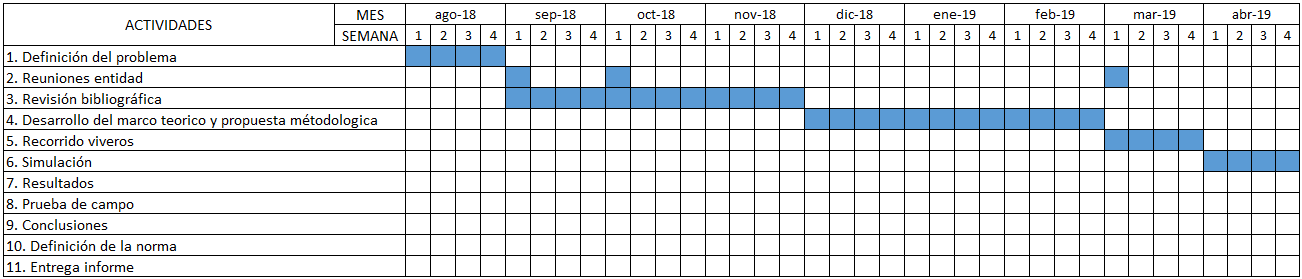
\includegraphics[width=12.75cm]{IMAGENES/CR1.png}
        \label{figura1}
\end{figure}
\begin{figure}[!h]
        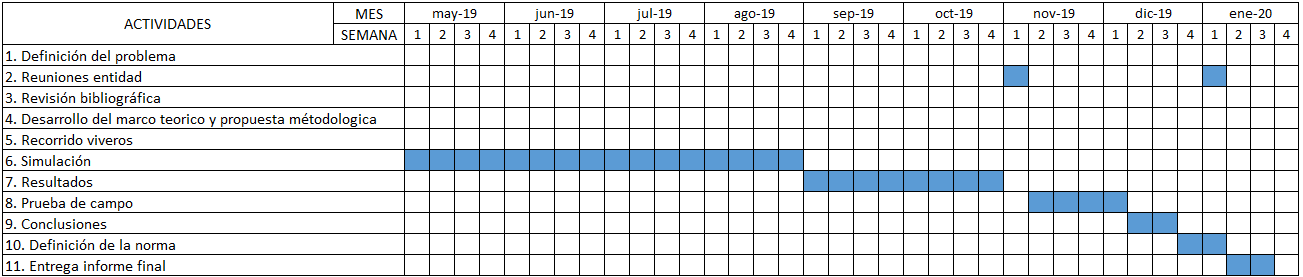
\includegraphics[width=12.75cm]{IMAGENES/CR2.png}
        \label{figura1}
\end{figure}

}
\end{frame}

\section{Presupuesto}
\begin{frame}
\frametitle{Presupuesto}
\begin{figure}[!h]
        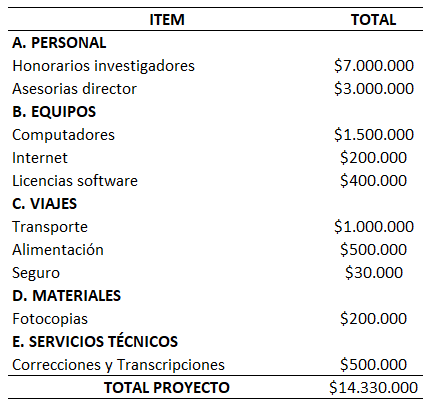
\includegraphics[width=8cm]{IMAGENES/PR.png}
        \label{figura1}
\end{figure}
\end{frame}



\bibliographystyle{plain}
  \bibliography{references}
\end{document}
